\documentclass[12pt]{article}

\usepackage[utf8]{inputenc}
\usepackage[T2A]{fontenc}
\usepackage[english]{babel}
\usepackage{amssymb}
\usepackage{graphicx}
\usepackage{float}
\graphicspath{ {images/} }

\textwidth=431pt
\textheight=600pt
\hoffset=-15pt
\voffset=-15pt

\usepackage{graphicx}
\usepackage{amsmath}
\makeatletter
\renewcommand{\@oddhead}{%
\vbox{%
\hbox to \textwidth{\strut \textit{CV, Assignment 3, Usvyatsov Mikhail} \hfill }
\hrule
\vspace{12pt}
}}
\renewcommand{\@oddfoot}{}
\makeatother

\begin{document}
	\bigskip
	\textbf{Algorithm}
	
For every composite image  we split it to images of every sign candidate;
And for every of sign candidates:\\
	\begin{enumerate}
		\item Clear the noise with Gaussian filter;
		\item Convert image to grayscale;
		\item Normalize histogram;
		\item Dilate;
		\item Extract edges with Canny;
	\end{enumerate}
	
	For every known sign we extract its edges and then make chamfer matching with cleared edges. Moreover, we have to choose the best match via score of matching.
	
	\textbf{Illustration}
	
	Here are a few results of image processing:\\
	
	\begin{figure}[H]
		\centering
		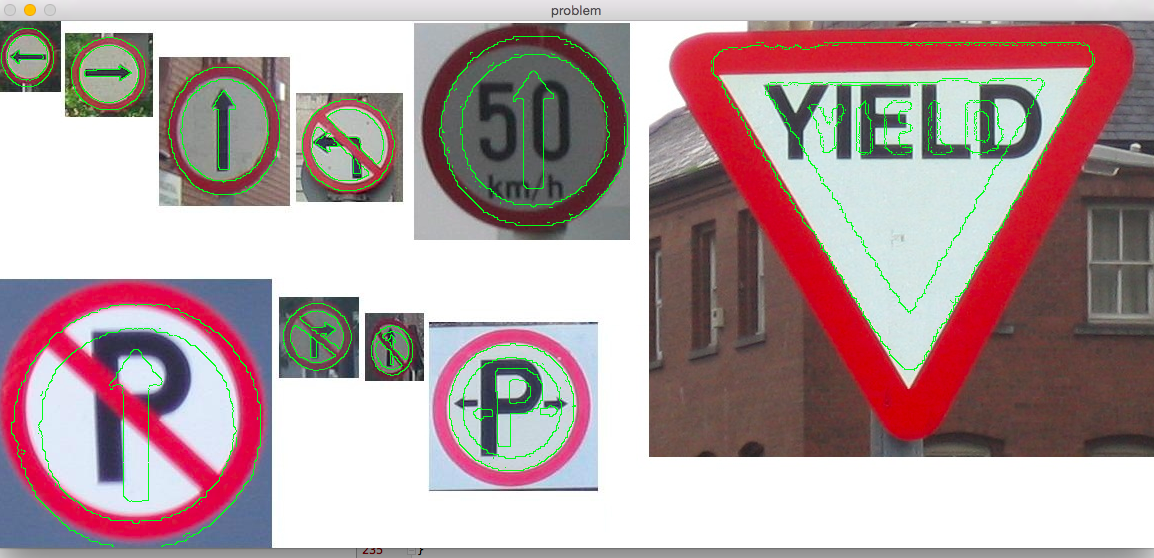
\includegraphics[width=15cm]{1}
		\caption{"Result of composite 1"}
	\end{figure}
	
	\begin{figure}[H]
		\centering
		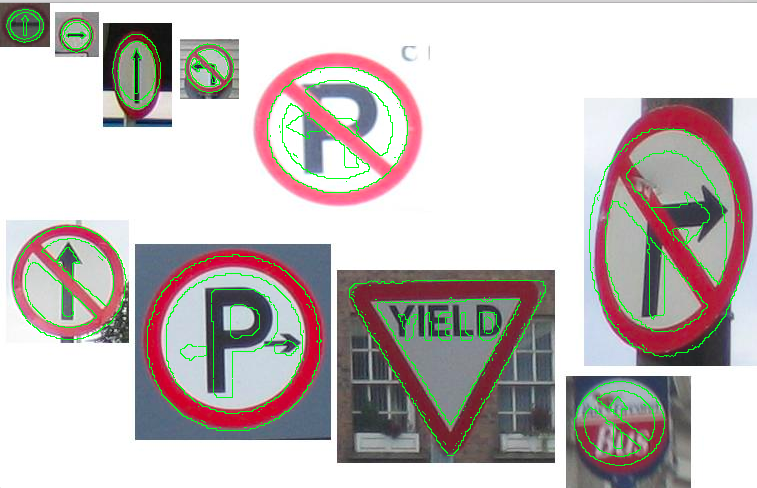
\includegraphics[width=15cm]{2}
		\caption{"Result of composite 2"}
	\end{figure}
	
	\medskip
	
	\textbf{Performance measure}
	According to confusion matrix:
	
	\begin{tabular}{|c||c|c|c|}
		\hline
		\ & predicted 1 & predicted 0 & Total \\
		\hline
		real class 1 & True Positive (TP) & False Negative (FN) & P\\
		\hline
		real class 0 & False Positive (FP) & True Negative (TN) & N \\
		\hline
		Total & $P'$ & $N'$ & $P+N$\\
		\hline 
	\end{tabular}
	\medskip
	
	The formulas for precision, recall and accuracy:
	\newcounter{ecounter}
	\begin{list}{\arabic{ecounter})~}{\usecounter{ecounter}}
		\item $precision = \dfrac{TP}{TP+FP}$
		\item $recall = \dfrac{TP}{P}$
		\item $accuracy = \frac{TP+TN}{P+N}$
	\end{list}
	
	The results of the program:

	precision =80 \%\\ 
	recall = 80\%\\
	accuracy = 95.5\%\\
	
	The problem was to detect mismatching. All the errors goes from mismatched signs.
	
\end{document}